\chapter{System Design}
\label{chap:system-design}

\section{Design Philosophy}
The distributed networked system is designed to address a long standing challenge in PRA: a fragmented software ecosystem. PRA studies often depend on many specialized quantification tools written in different languages (e.g., C++, Erlang) and distributed as standalone desktop applications. Rewriting these solvers into a single unified codebase is costly and time intensive. Instead, the guiding idea of this work is to wrap and orchestrate existing tools so they can be used together as scalable network services.

To achieve this, the system combines three of the well established architectural patterns mentioned in ~chapter \ref{chap:distributed-systems}:

\begin{itemize}
    \item \textbf{Microservices:} PRA solvers are packaged and operated as independent services that can be deployed and scaled.
    \item \textbf{Event driven execution:} Jobs are handled asynchronously. Submitting a job generates internal events (e.g., queued, started, completed, failed) so that work can be scheduled, retried, and monitored without tight coupling between the request interface and the compute workers.
    \item \textbf{Client-Server:} Users and applications act as clients that submit quantification requests to a central service endpoint. Users can submit jobs, see the job status and retrieve the quantification results from databases.
\end{itemize}

The architecture maintains a clear separation between the control plane and the data plane. The control plane provides the externally visible interface (job submission, status queries, and administration) and performs orchestration tasks such as routing, scheduling, and tracking job state. The data plane focuses on raw computation, where worker processes execute solver runs and produce artifacts (logs, intermediate files, and results). This separation makes it easier to scale computation independently of the user facing services and provides a natural structure for monitoring and operational control.

All services are exposed through HTTP/REST APIs, which act as a practical universal adapter. A language agnostic interface like this allows any client from a legacy program to a modern web frontend, to submit jobs and retrieve results using a common protocol. This turns PRA quantification tasks into web accessible utilities.

Finally, the system uses containerization rather than full virtual machines to manage solver dependencies and ensure reproducible execution. Each solver and its runtime requirements are packaged into a container, reducing environment conflicts and eliminating the "works on my machine" problem. Containers are lightweight enough to launch on demand, enabling many solver instances to run in parallel when resources are available. In this way, legacy desktop tools can be transformed into scalable, network accessible services without modifying their internal source code.

\section{Core System Components}
The system consists of several key components:

\begin{itemize}
    \item \textbf{Reverse Proxy / Load Balancer}: in an on-premise cluster setup, the reverse proxy works an intermediary server positioned in front of the internal services that intercepts client requests, forwards them to the backend server, and returns the response as if it originated from the proxy itself, enhancing security by hiding the backend's IP address while also improving performance through balancing traffic. In a single node distributed memory setup, the load balancer distributes incoming requests across multiple service instances running on the machine.
    \item \textbf{API Gateway}: provides the public REST interface. It is responsible for user facing concerns such as authentication, request validation, and consistent request/response formatting. The gateway hides internal implementation details so clients can submit jobs and query results through a stable API.
    \item \textbf{Business Logic Service}: implements the core application workflow. It handles operations such as job submission, job status queries, retrieval of results, and returning error messages and logs when runs fail. This layer also manages job metadata (e.g., identifiers, timestamps, priorities, and solver selection) and coordinates with the queueing and storage components.
    \item \textbf{Task Producer}: converts user requests into structured, queueable task messages that can be placed into the message broker for asynchronous execution. It assigns the requests to queues based on analysis type and priority.
    \item \textbf{Message Broker}: is the communication backbone of the system. It provides queues that decouple job submission from job execution, enabling asynchronous processing and higher throughput under multi user demand.
    
    %The broker persists messages and supports retry mechanisms so tasks are not lost during transient failures or service restarts.
    
    \item \textbf{Worker Pools}: provide the compute layer. Workers consume tasks from the message broker and run the requested PRA computations. Each worker runs in an isolated, self contained environment (typically containerized) that includes the required solver binaries and dependencies. This design improves reproducibility, supports parallel execution at scale, and prevents one job from corrupting another job's runtime environment. Workers also report health and execution status so the control plane can detect failures and reschedule work when needed.
    \item \textbf{Object Storage}: stores inputs and outputs such as models, intermediate artifacts, final results, and per task logs.
\end{itemize}

Figure~\ref{fig:system-design} summarizes the workflow of the proposed system. Client requests first enter through a reverse proxy or a load balancer, depending on whether the deployment is on-premise cluster based or single node based. The proxy forwards the requests to the API gateway. For quantification jobs, the producer converts the request into a message and places it in the message broker queue. Worker pools then consume messages from the queue, execute the tasks, and forward the results and logs. These forwarded results and logs are then stored in object storage for later retrieval. For requests that are not quantification jobs, the business logic handles them directly by retrieving the job status or the result or the error log (depending on the request's demands) and returning the response to the user.

\begin{figure}[]
  \centering
  \includesvg[width=\textwidth]{4-design/plots/system-design.svg}
  \caption{Workflow of the distributed networked system.}
  \label{fig:system-design}
\end{figure}

% Figure~\ref{fig:rest-api-architecture} shows a simplified REST based workflow for job submission and execution.
%\begin{figure}[h]
  \centering
  \begin{tikzpicture}[
      scale=0.8,
      >=stealth,
      box/.style={draw,rectangle,rounded corners=2pt,minimum width=2.2cm,
                  minimum height=0.8cm,align=center,fill=white,drop shadow},
      apibox/.style={draw,rectangle,rounded corners=3pt,minimum width=2.8cm,
                  minimum height=1cm,align=center,fill=blue!10,drop shadow},
      msg/.style={->, thick},
      label/.style={font=\small,draw=none}
    ]
    
    % Client
    \node[box] (client) {Client};
    
    % REST API Layer with its components
    \node[apibox, right=2cm of client] (api) {RESTful API Layer};
    \node[box, below=0.8cm of api] (auth) {Authentication \& Validation};
    
    % Publisher
    \node[box, right=3cm of api] (publisher) {Publisher};
    
    % Database
    \node[box, below=1cm of publisher] (db) {Distributed Databases};
    
    % Fit node for Backend System
    \node[fit=(api)(auth)(publisher)(db),
          draw, inner sep=0.3cm, dashed, 
          label={[yshift=0.3cm]\textbf{Backend System}}] (platform) {};
    
    % Draw connections
    \draw[msg] (client) -- node[above,label]{POST task} (api);
    \draw[msg] (api) -- node[above,label]{models} (publisher);
    \draw[msg] (api) -- node[below,label]{solver parameters} (publisher);

    % Two-way arrow between API and Auth
    \draw[<->, thick] (api) -- (auth);
    
    % Status monitoring path
    \draw[msg, blue] (api) to[bend right=30] node[above,label] {GET results} (client);
    
    % Database connections
    \draw[msg, blue] (db) -- node[right,xshift=0.8cm,label]{query results} (api);
    
  \end{tikzpicture}
  \caption{Simplified RESTful API architecture for the microservice.}
  \label{fig:rest-api-architecture}
\end{figure}

\section{Interoperability and Extensibility}
Through its API endpoints, the system exposes multiple established PRA solvers and provides a comprehensive list of quantification services. These services include probability calculation, cut set enumeration, common cause failure analysis, importance measures, safety integrity level assessment, and uncertainty quantification. To support these services, the architecture integrates multiple algorithmic engines and approximation methods, allowing the user to select the optimal computational path for their tasks based on model characteristics and performance requirements. Figure~\ref{fig:pracciolini} lists the tools supported by the interoperability layer and the model formats each tool uses.

\begin{figure}[]
  \centering
  \includesvg[width=\textwidth]{4-design/plots/pracciolini.svg}
  \caption{Example of supported model transitions in the operability layer.}
  \label{fig:pracciolini}
\end{figure}

The system achieves interoperability through a solver independent job specification that captures the essential parameters for PRA quantification. It includes the model reference, the analysis type, and the required outputs. Figure~\ref{fig:interoperability} shows the fields of this specification. This schema is called the \emph{intermediate JSON format}. Users can upload models in a tool specific format and select any supported solver. When a conversion path exists, the system converts the model to the format required by the chosen tool through this intermediate format behind the scenes.

\begin{figure}[]
  \centering
  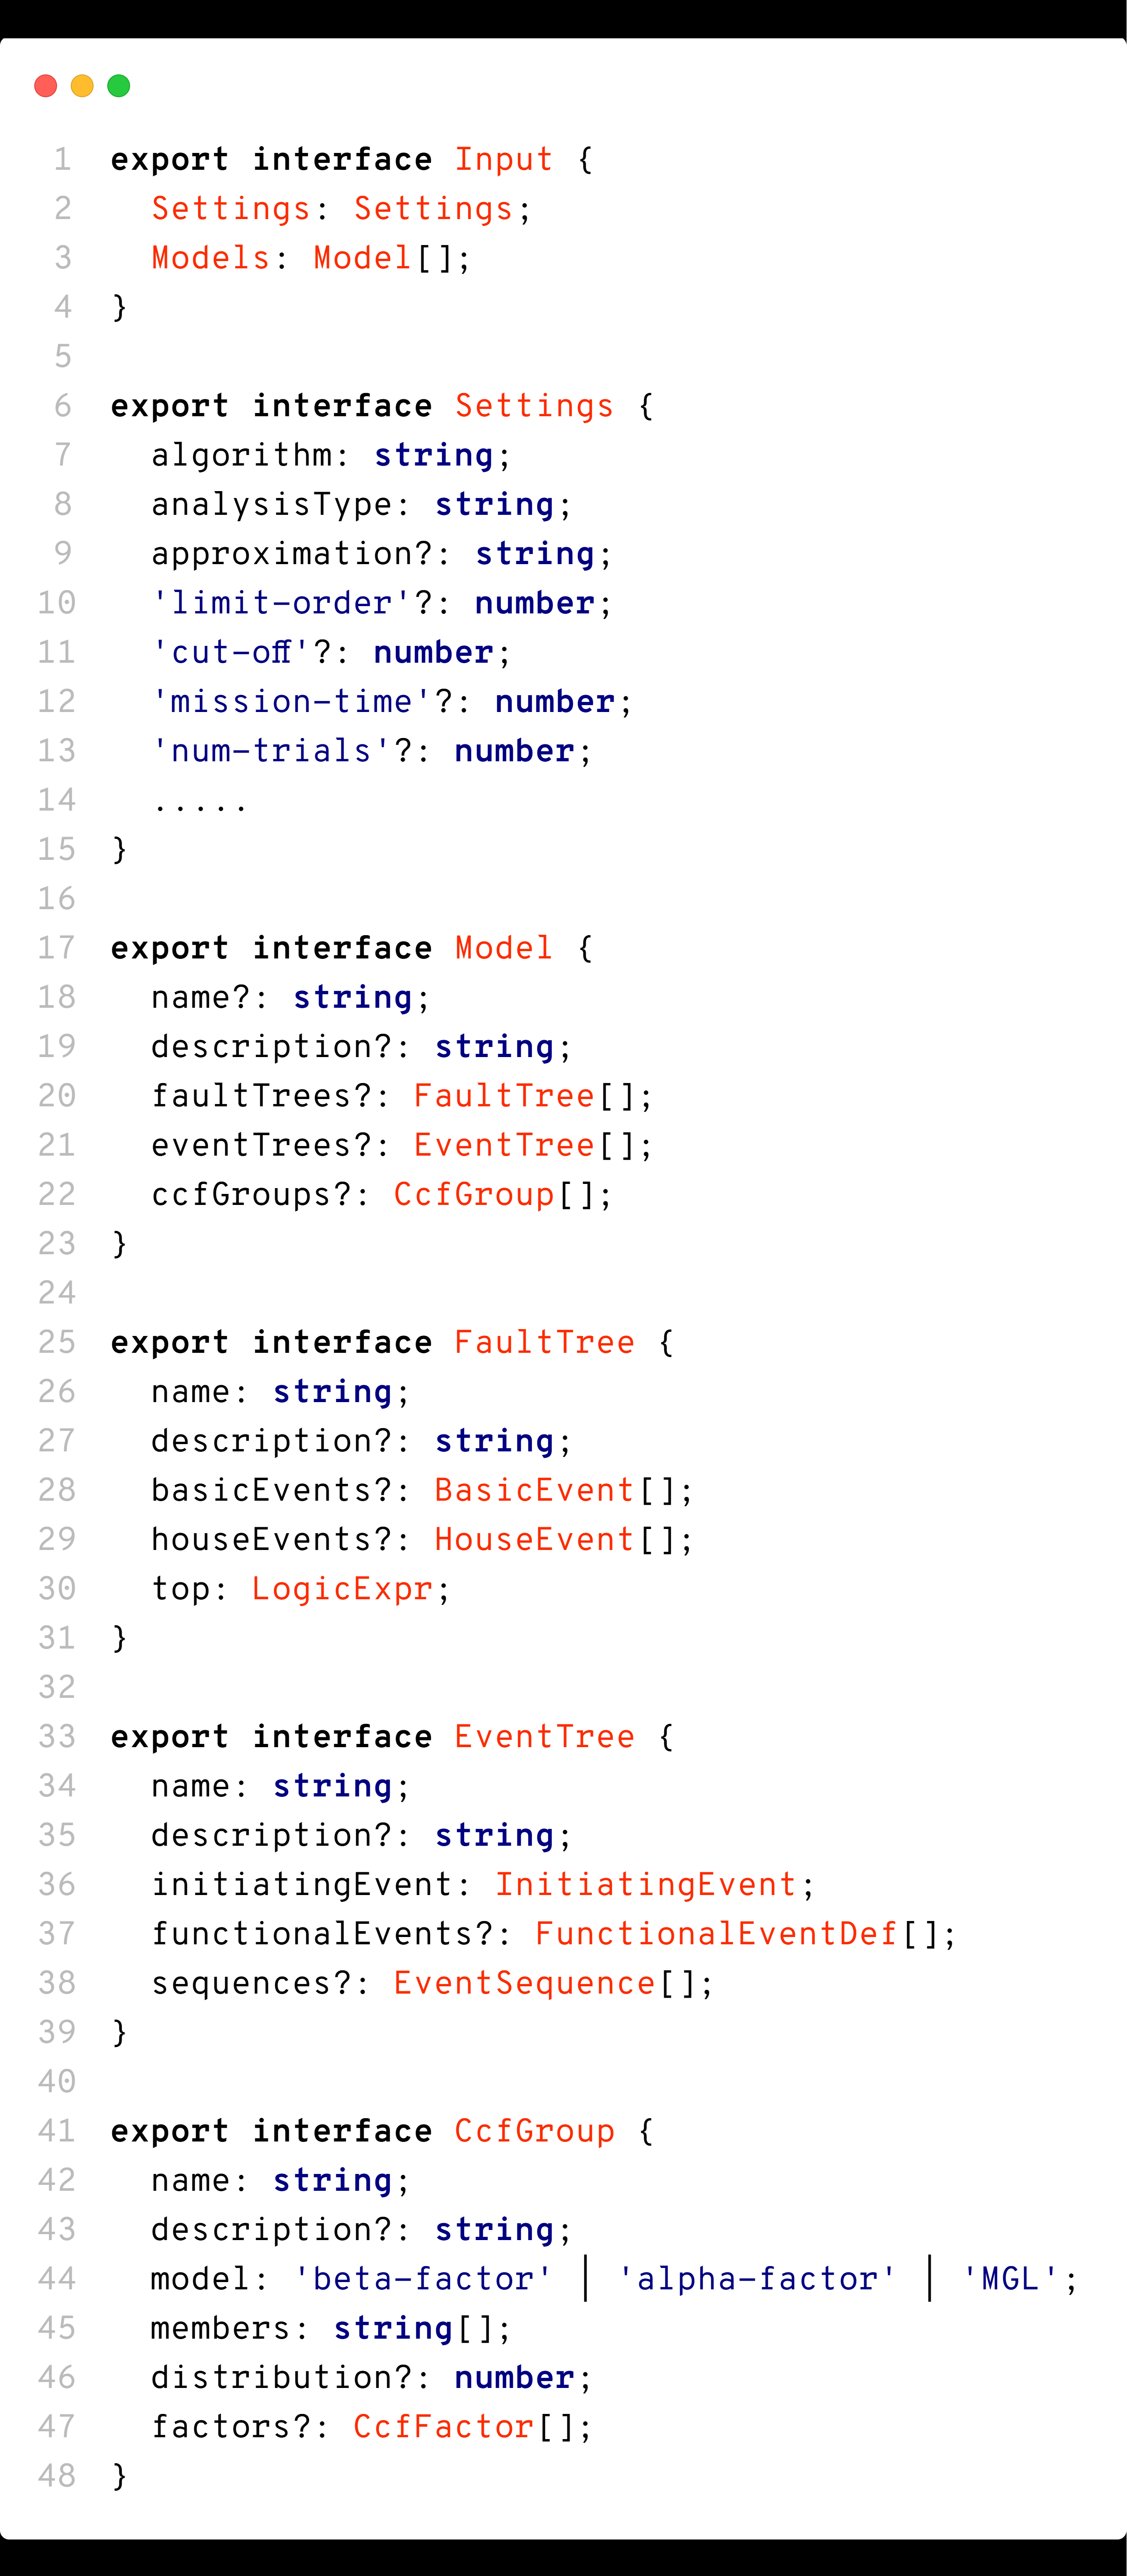
\includegraphics[width=0.60\linewidth]{4-design/plots/interoperability}
  \caption{Data structure of the intermediate JSON format.}
  \label{fig:interoperability}
\end{figure}

The architecture supports schema evolution through versioned interfaces, maintaining backward compatibility while enabling forward progress. All external interfaces are versioned, allowing the system to translate between different specification versions and ensuring existing workflows continue to function as the platform evolves to incorporate new computational approaches and data formats.

\section{Performance Optimization Strategies}
The system employs multiple queues to match workload characteristics, including first-in-first-out for fairness and priority queues for time sensitive computations. Work stealing improves resource utilization by allowing underutilized workers to claim tasks from overloaded queues.

Large models are parallelized differently depending on whether the analysis tool is closed source or open source. For closed-source tools, optimization of the internal algorithms is not feasible. Consequently, the only practical approach is to modify the input model. In this approach, an event tree can be dissociated into individual event sequences, after which each sequence is queued and quantified as a separate job. For open-source tools, more efficient code-level optimizations can be implemented. Rather than creating a separate representation for every dissociated input, a probabilistic directed acyclic graph (PDAG) is constructed only once for each event tree, and different parts of that PDAG are then distributed as separate jobs. This avoids repeatedly constructing equivalent PDAGs and significantly speeds up processing. In addition, the workflow uses adaptive quantification: an initial estimate of the sequence frequency is obtained using BDD based or Monte Carlo methods, and then cut sets are enumerated only up to a specified frequency truncation limit using internal algorithms. In this adaptive approach, cut sets are enumerated using ZBDD when following the BDD based path, and using MOCUS when following the Monte Carlo path.

This decomposition extends to importance measures, where basic event based analyses are queued separately, and uncertainty quantification, where each simulation run becomes an independent job. All results are aggregated deterministically using predefined output formats that specify the necessary data fields for reconstruction.

\section{Fault Tolerance Mechanisms}
The system ensures reliability through multiple approaches. Computational components employ a stateless design, allowing any worker to process tasks without storing any internal session data. As a result, the system can recover quickly by redirecting the jobs to healthy instances. Cascading failures are prevented by isolating degraded services and returning graceful error messages until these services recover.

Message processing guarantees at-least-once delivery, with idempotent operations ensuring duplicate messages are processed only once. Workers acknowledge messages only after successfully persisting results, while unacknowledged messages are automatically re-queued after configurable timeouts.

Health monitoring continuously checks components through regular ping intervals, triggering automatic remediation actions such as restarting failed containers to maintain system availability.

In addition, the system employs an exponential backoff reconnection strategy to handle message broker failures or restarts, retrying up to three times to reconnect. If reconnection is unsuccessful, the message is routed to the dead letter queue. Each message also includes a configurable time-to-live (TTL): if a worker cannot complete a quantification within the TTL window (default: 1 hour), the message expires and is moved to the dead letter queue to avoid saturating workers with stalled or long running tasks. Users may override the default TTL to control the maximum allowable processing time for their requests.

\section{Resource Management and Scalability}
The system’s resources are not auto scaled in response to workload. Instead, an administrator can scale the deployment up or down using the provided scripts: horizontally by adding or removing worker nodes in an on-premise cluster deployment, and vertically on a single node by increasing available resources through running multiple service instances across the node’s virtual CPUs (and GPUs where available).

A multi tenant resource model promotes fair usage through per-user quotas and queueing controls. Each user is subject to an individual request rate limit (default: 10 requests per hour) and a storage limit (default: 100 GB per user). The queueing system also supports priorities, but these priorities are not inferred automatically, jobs are ordered and processed according to the priority explicitly set by the user.

Hardware support depends on the deployment mode. Single node deployments can use both CPU and GPU capable workers, enabling GPU acceleration where applicable, while on-premise cluster deployments currently support CPU only workers. As a result, GPU execution is available only in the single node configuration, whereas cluster executions run entirely on CPU resources.

\section{Security and Access Control}
Authentication uses token based credentials validated with each request. Authorization follows the principle of least privilege through role based access control combined with attribute based policies. These policies grant access to proprietary tools only to licensed users, while unlicensed users are limited to open-source alternatives.

Multi tenancy ensures isolation between user environments, preventing unauthorized access to data or computational resources. Complete audit trails record all significant actions including model submissions and result accesses.

Data compression at client-server interfaces serves dual purposes: protecting sensitive nuclear facility data and compressing large input/output files to reduce storage usage.

\section{Operational Simplicity and Maintainability}
Operational simplicity is achieved through platform-as-code (PaaS) principles that enable reproducible deployments across all environments, supported by automated scaling for both planned expansion and emergency recovery.

Comprehensive monitoring is built into the architecture, with each component emitting standardized metrics, logs, and traces. The system tracks queue lengths, processing times, error rates, and resource utilization, providing real-time visibility into system health with automated alerting for anomalous conditions.

Detailed documentation covers API usage guidelines, deployment procedures, and implementation workflows through comprehensive markdown files and operational guides. The system also includes extensive test suites with both end-to-end integration tests and functional unit tests to verify system behavior.
